\documentclass{article}

% Package necessari
\usepackage[a4paper]{geometry}
\usepackage[utf8]{inputenc}
\usepackage[english]{babel}
\usepackage[T1]{fontenc}
\usepackage[font={small,sl}]{caption}
\usepackage[font={small,sl}]{subcaption}
\usepackage{graphicx}
\usepackage[usenames, table, dvipsnames]{xcolor}
\usepackage{hyperref}
\usepackage[most]{tcolorbox}
\usepackage[section]{placeins}
\usepackage{soulutf8}
\usepackage{listings}
\usepackage{tabularray}
\usepackage[toc,page]{appendix}


% Titolo del documento
\title{\small Report of "Network \& System defense" project \\
\Huge \textbf{MLKM SHIELD}\\
\Large (Protection against malicious LKM)}

% Autore del documento
\author{Simone Tiberi (M. 0299908)\\%
(email: \texttt{\href{mailto:simone.tiberi.98@gmail.com}{simone.tiberi.98@gmail.com}})}

% Data del documento
\date{\today}

% Impostazione delle lunghezze di alcuni elementi del documento
\setlength{\parskip}{1em}
\setlength{\parindent}{0em}

% Impostazioni del package hyperref
\hypersetup{
        colorlinks=true,
        linktocpage=true,
        linkcolor=blue,
        urlcolor=blue,
        citecolor=blue,
        pdftitle={Relazione progetto NSD},
        pdfauthor={Simone Tiberi},
}

% Tokyonight colors
\definecolor{tn-bg}{HTML}{24283b}
\definecolor{tn-terminal}{HTML}{414868}
\definecolor{tn-red}{HTML}{f7768e}
\definecolor{tn-fg}{HTML}{c0caf5}
\definecolor{tn-fg-dark}{HTML}{a9b1d6}
\definecolor{tn-green}{HTML}{9ece6a}
\definecolor{tn-comment}{HTML}{565f89}
\definecolor{tn-blue0}{HTML}{3d59a1}
\definecolor{tn-blue}{HTML}{7aa2f7}
\definecolor{tn-cyan}{HTML}{7dcfff}

\lstset{
	language=C,
	frame=shadowbox,
    backgroundcolor=\color{tn-bg},
	rulesepcolor=\color{tn-terminal},
    basicstyle=\color{tn-fg}\ttfamily\scriptsize,
	keywordstyle=\color{tn-red}\bfseries\scriptsize,
	stringstyle=\color{tn-green}\scriptsize,
	commentstyle=\color{tn-comment}\scriptsize,
	numbers=left,
	numberstyle=\tiny\color{tn-fg-dark},
	numbersep=5pt,
	tabsize=2,
	showtabs=false,
	showspaces=false,
	showstringspaces=false,
	escapechar=|,
	captionpos=b,
	breaklines=true,
	keepspaces=true
}

\graphicspath{ {./figs/} }

\newtcolorbox{custombox}[1]{
	colframe  = blue!25,
    colback   = blue!10,
    coltitle  = blue!20!black,
    title     = #1,
	fonttitle = \bfseries,
    breakable,
    enhanced,
}

\newcommand{\terminal}[1]{\colorbox{tn-bg}{\textcolor{tn-fg}{\texttt{#1}}}}

\begin{document}
\maketitle
\tableofcontents
	\section{Project specification}
	This project entails writing some protection mechanism in the Linux kernel (as a patch, a security module, a simple
	module, \dots) to prevent malicious loadable kernel modules to tamper with internal data structures of the kernel.

	In particular, beyond the example that we have discussed in class, it is possible that a module will not perform
	any attack during the loading phase, but it will perform some form of delayed attack (e.g., by relying on a
	Tasklet). Your scheme should also be able to perform this kind of detection.

	If a module is detected as malicious, it must be unmounted, and any possible side effect generated by it should be
	reverted.

	\section{Project structure}
	\begin{custombox}{Repository}
		Link to Github repository: \url{https://github.com/tibwere/mlkm-shield}
	\end{custombox}

	The project is organized into several files, each of which contains stuffs relating to certain components of the
	project (e.g. hooks, \textit{machine-specific} operations, \dots).

	The following sections are aimed at describing each component of the module developed, by analyzing core data
	structures and procedures implemented, as well as the general idea behind the functioning of the module.

	\section{Introduction to LKM monitoring}
	The protection mechanism is based on the assumption that when the shield module is mounted, the memory is in a
	\textit{good} state. As a matter of fact, in the beginning of the installation process the state of the critical
	memory areas is \textbf{cached}.

	Another assumption is that the areas to be protected are immutable over time and therefore it is not necessary to
	update the caching status from time to time at each execution of the modules under analysis.

	The areas considered critical and therefore monitored by the shield module are:
	\begin{itemize}
		\item \textbf{System call table}, because a rootkit can change some function pointers within the table and thus
		change the behavior of certain system calls,
		\item \textbf{IDT} (\textbf{I}nterrupt \textbf{D}escriptor \textbf{T}able), because a rootkit can modify
		interrupt handlers to perform malicious activity,
		\item a list of \textbf{additional symbols} that the sysadmin can specify inside a configuration file
		(sec.~\ref{sec:config}) before mounting the shield module.
	\end{itemize}

	Taking advantage of the \texttt{kretpobe} (and also \texttt{kprobe}) mechanisms offered by Linux
	Kernel, the very last function invoked by the kernel inside the mounting process is hooked, so
	that after the return statement, a \textbf{verification step} can begin (fig.~\ref{fig:monitoring}).

	\begin{figure}[!htbp]
		\centering
		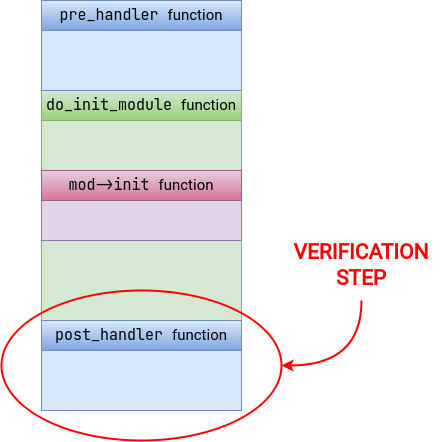
\includegraphics[scale=0.4]{monitoring}
		\caption{Hook scheme for \texttt{do\_init\_module}}
		\label{fig:monitoring}
	\end{figure}

	Obviously, using only this mechanism, a condition like the following one could occur:
	\begin{itemize}
		\item a non-malicious module $A$ is running a function $\alpha$,
		\item a malicious module $B$ is running \ul{concurrently} (such as shown in fig.~\ref{fig:concurrency}) a
		function $\beta$,
		\item the shield module recognize $A$ as malicious \ul{and also $B$ as non-malicious} thus \textbf{making two
		mistakes}.
	\end{itemize}

	\begin{figure}[!htbp]
		\centering
		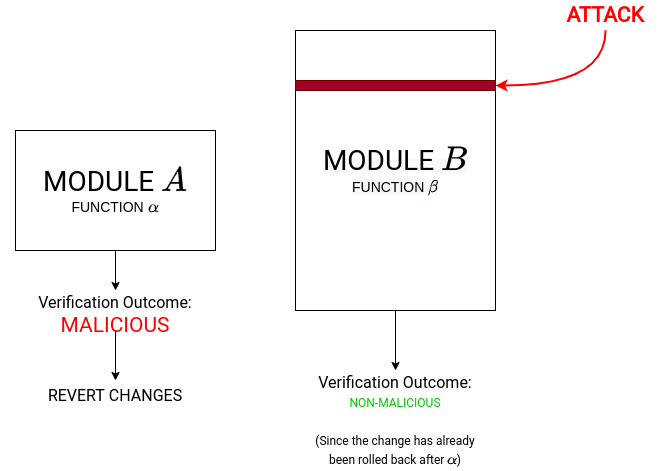
\includegraphics[scale=0.4]{concurrency}
		\caption{Detection scheme problem without using IPI}
		\label{fig:concurrency}
	\end{figure}

	For this reason the use of IPI has been introduced to ensure that:
	\begin{itemize}
		\item in the \textbf{pre-handler}, the core that is performing the mount of the module (in an non-preemptible
		way), requires the others to spin on a certain barrier variable,
		\item in the \textbf{post-handler}, the same core as before changes the value of the barrier variable, thus
		allowing the restoration of normal activity.
	\end{itemize}

	Finally, for the detection of malicious actions in deferred mode, the probe mechanism was exploited again, this
	time dynamically hooking functions inside the modules, as described in detail in the section ~\ref{sec:hooks}.

	\section{Components description}

	\subsection{"Black/White list" component}\label{sec:bwlist}
	This component simply contains a function and a couple of macros for inserting modules into the black / white list.
	These two lists allow to realize the following mechanisms:
	\begin{itemize}
		\item a module present in the \textbf{white list} is considered \textit{a priori} not malicious and therefore
		is not subject to monitoring, which implies that it will not be damaged in terms of performance due to the use
		of kretprobes,
		\item a module present in the \textbf{black list} is considered \textit{a priori} malicious and therefore is
		removed directly. In sec.~\ref{sec:hooks} it will be showed the mechanism used to safely remove this kind of
		module without risking \texttt{SEGFAULT} or execution of malicious code.
	\end{itemize}

	\subsection{"Configuration" component}\label{sec:config}
	\textbf{"Configuration"} is a component in which there are defined a few variables that a sysadmin can change to
	tune the shield module according to his needs. In particular there are:
	\begin{itemize}
		\item two boolean variables to decide whether or not to secure system call table and IDT respectively,
		\item the list of additional symbols to protect, \ul{where you do not have to specify the address directly},
		but the name of the symbol, readable from \texttt{/proc/kallysms},
		\item a white list of modules not to be monitored, because they are considered not malicious \textit{a priori},
		\item a black list of modules to be considered malicious \textit{a priori} and therefore not to be mounted.
	\end{itemize}

	\subsection{"Safe memory" component}
	\textbf{Safe memory} is one of the core components of the module. Inside, it is defined the data structure
	\texttt{safe\_area} (list.~\ref{lst:safe-area}), which is the logical representation of the caching of the state of
	a specific \textit{quad word} (\texttt{64 bits}) in memory.

	Inside the module three different arrays of \texttt{safe\_area} structures are used:
	\begin{itemize}
		\item one for system call table function pointer, of size \texttt{NR\_syscalls},
		\item one for IDT, seen as a sequence of unsigned long which implies that the size of array is evaluated as:
		\begin{equation*}
			\dfrac{\mathtt{IDT\_ENTRIES} \cdot \mathtt{sizeof(gate\_desc)}}{\mathtt{sizeof(unsigned long)}}
		\end{equation*}
		\item one for the list of additional symbols specified inside the array in the configuration file.
	\end{itemize}

	One of the main functions defined in this module is \texttt{verify\_safe\_areas} used in a lot of handlers defined
	into the \textbf{"Hooks"} component. Inside, \texttt{inspect\_sa} is called for each array to check if critical
	memory areas have been altered. In this case:

	\begin{itemize}
		\item a new threat is added to the \texttt{/sys} audit (sec.~\ref{sec:threats}),
		\item the hacked memory area is restored, after disabling the memory protection by overwriting the \texttt{CR0}
		register (sec~\ref{sec:x86}),
		\item the malicious module is removed (sec. ~\ref{sec:shield}).
	\end{itemize}

	\subsection{"Shield" component}\label{sec:shield}
	Inside the \textbf{shield} component are defined two core structures for the functionality of the module:
	\begin{itemize}
		\item \texttt{monitored\_module} which contains metadata used to monitor the module, such as the reference to
		the \texttt{struct module}, a boolean value used to avoid nested verifications, and two set of pointers used to
		realize two different linked lists:
		\begin{itemize}
			\item the former links together all monitored modules,
			\item the latter links a monitored module to the kretprobes hooked to its own functions.
		\end{itemize}

		\item \texttt{module\_probe} which represents a kretprobe hooked to a specific function of the module, so
		inside of it there are the reference to the owner (\texttt{struct monitored\_module}), the kretprobe itself and
		finally a couple of pointers used to link all the probes related to the same module together and to the owner
		too.
	\end{itemize}

	In list.~\ref{lst:shield-structs} are shown these structures and furthermore in fig..~\ref{fig:shield-structs} is
	represented how thy are linked together.

	\begin{figure}[!htbp]
		\centering
		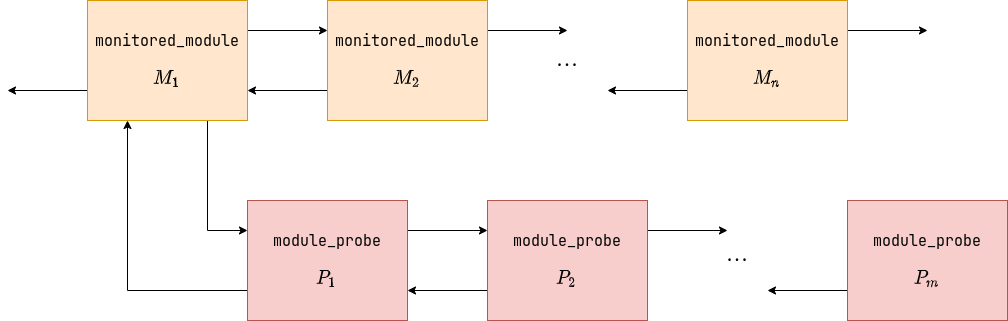
\includegraphics[scale=0.4]{shield-structs}
		\caption{Relationship between \texttt{monitored\_module} and \texttt{module\_probe}}
		\label{fig:shield-structs}
	\end{figure}

	Inside this component is defined also a parameter of the module, that is the \texttt{removed} variable. Moment by
	moment is it possible to see how many modules have been detected as malicious reading the content of
	\texttt{/sys/module/mlkm\_shield/parameters/removed} pseudo-file.

	An interesting function defined inside this module is \texttt{remove\_malicious\_lkm}. To remove a module you need
	to use the function \texttt{free\_module}, which is not exported by default for module programming. For this
	reason, using a function defined inside the \textbf{symbols} component (sec.~\ref{sec:symbols}) its address has
	been retrieved.

	\subsection{"Symbols" component}\label{sec:symbols}
	In the \textbf{symbols} component are defined some utility functions used by other ones, such as:
	\begin{itemize}
		\item \texttt{symbol\_lookup}, which allows you to retrieve the address of a symbol in the kernel memory space
		specifying its name. To do this you need to use the \texttt{kallsyms\_lookup\_name} function, which is no
		longer available for module programming starting with kernel 5.7, so the kprobing mechanism was used to
		retrieve its address,
		\item \texttt{get\_system\_call\_table\_address}, which by relying on the previous one, lets you to retrieve
		the address of the system call table. Up to version 4.4 of Linux, the search is carried out according to a
		brute force approach, starting from the address of \texttt{the sys\_close} system call\footnote{For
			conventional Linux Kernel builds, this address is lower than the system call table one.},
		\item \texttt{get\_idt\_address}, which allows you to retrieve the base address of the IDT, by relying on the
		\texttt{SIDT} instruction wrapped into the
		\href{https://elixir.bootlin.com/linux/latest/source/arch/x86/include/asm/desc.h#L223}{\texttt{store\_idt}} API
		of the kernel
	\end{itemize}

	\subsection{"Machine specific (x86)" component}\label{sec:x86}
	This component simply contains a function and a couple of macros to modify \texttt{CR0} register to enable/disable
	memory protection. For all this we change the bit \texttt{X86\_CR0\_WP} using \texttt{memory} clobber to avoid
	compile-time instruction reordering (according to
	\href{https://elixir.bootlin.com/linux/v5.17.3/source/arch/x86/include/asm/special_insns.h#L54}{this}
	implementation).

	As you can see by analyzing the source code, the module uses machine-specific facilities for x86, so for a possible porting to other architectures it would be necessary to define additional header files in the \texttt{asm} directory and different implementations of the API C using \texttt{\#define CONFIG\_XXX} directives.

	\begin{appendices}
		\section{Source codes mentioned in the document}
		\lstinputlisting[
			caption={\texttt{safe\_area} struct},
			label={lst:safe-area},
			escapechar=,
			firstline=31,
			lastline=40
		]{../include/safemem.h}

		\lstinputlisting[
			caption={\texttt{monitored\_module} and \texttt{module\_probe} structs},
			label={lst:shield-structs},
			escapechar=,
			firstline=23,
			lastline=54
		]{../include/shield.h}
	\end{appendices}

\end{document}
